\documentclass{beamer}
\usepackage[brazilian]{babel}
\usepackage[utf8]{inputenc}
\usepackage{calc}
\usepackage[absolute,overlay]{textpos}
\mode<presentation>{\usetheme{tud}}

\title[JEWEL]{JEWEL}
%\subtitle
\institute[HEPIC-Instituto de Física]{HEPIC-Instituto de Física}
\author{Fabio Canedo}
\date{\today}

% Insert frame before each subsection (requires 2 latex runs)
\AtBeginSubsection[] {
	\begin{frame}<beamer>\frametitle{\titleSubsec}
		\tableofcontents[currentsection,currentsubsection]  % Generation of the Table of Contents
	\end{frame}
}
% Define the title of each inserted pre-subsection frame
\newcommand*\titleSubsec{Content}
% Define the title of the "Table of Contents" frame
\newcommand*\titleTOC{Content}

% define a symbol which can be removed if you don't need it
\newcommand{\field}[1]{\mathbb{#1}}
\newcommand{\Zset}{\field{Z}}

\begin{document}

{
% remove the next line if you don't want a background image
\usebackgroundtemplate{}%
\setbeamertemplate{footline}{\usebeamertemplate*{minimal footline}}
\frame{\titlepage}
}

{\setbeamertemplate{footline}{\usebeamertemplate*{minimal footline}}
\begin{frame}\frametitle{\titleTOC}
	\tableofcontents
\end{frame}
}

\section{First Remarks}
\subsection{About the cross-section}

\begin{frame}\frametitle{About the cross-section}

	About the cross-section presented on last meeting:
	\pause
	\begin{equation}
	\sigma_i(E,T)=\int_{0}^{|\hat{t}|_{max}(E,T)}d|\hat{t}|\int_{x_{min}(|\hat{t}|)}^{x_{max}(|\hat{t}|)} dx \sum_{j \in \{ q,\overline{q},g\}} f_{j}^{i}(x,\hat{t})\frac{\mathrm{d}\sigma}{\mathrm{d}\hat{t}}(x\hat{s},|\hat{t}|)
	\end{equation}
	\pause
	Here $E$ stands for the parton energy and $T$ for the local temperature.
	$\hat{s}$ is the center of mass energy of the scattering center plus propagated parton system.
	$\hat{t}$ stands for the propagated parton current virtuality.
\end{frame}

\section{Background Subtraction}

\begin{frame}\frametitle{4-Momentum Subtraction}

	JEWEL authors studied 2 ways of proceding on the background subtraction procedure:
	\begin{itemize}
		\item 4-Momentum Subtraction;
		\item Grid Subtraction 1;
		\item Grid Subtraction 2;
	\end{itemize}

\end{frame}

\subsection{4-Momentum}

\begin{frame}\frametitle{4-Momentum}
	\begin{itemize}
	\item Cluster initial jet collection.
	\item Compile a list of thermal momenta.
	\item For each jet, get list of thermal momenta that have $\Delta R < 1\times 10^{-5}$ with a jet constituent.
	\item Sum the list's four-momenta.
	\item Subtract it from jet four-momenta.
	\end{itemize}
\end{frame}

\subsection{Grid Sub 1}

\begin{frame}\frametitle{Grid Sub 1}
	\begin{itemize}
	\item Cluster initial jet collection.
	\item Compile a list of thermal momenta.
	\item Define a grid resolution and place it over jets. 
	\item Sum the list's four-momenta of both thermal and jet constituent in each cell.
	\item Subtract thermal four-momenta from jet constituent four-momenta.
	\item Re-cluster jet.
	\end{itemize}
\end{frame}
\subsection{Grid Sub 2}

\begin{frame}\frametitle{Grid Sub 2}
	\begin{itemize}
	\item Compile a list of thermal momenta.
	\item Define grid resolution over entire event.
	\item Sum the list's four-momenta of both thermal and every particle(non-thermal) in each cell.
	\item Subtract thermal four-momenta from "normal" four-momenta.
	\item Cluster jet.
	\end{itemize}
\end{frame}

\section{Preliminary Results}
\subsection{Jet shape}

\begin{frame}\frametitle{Preliminary Results}

        
        \begin{minipage}{1.0\textwidth}
		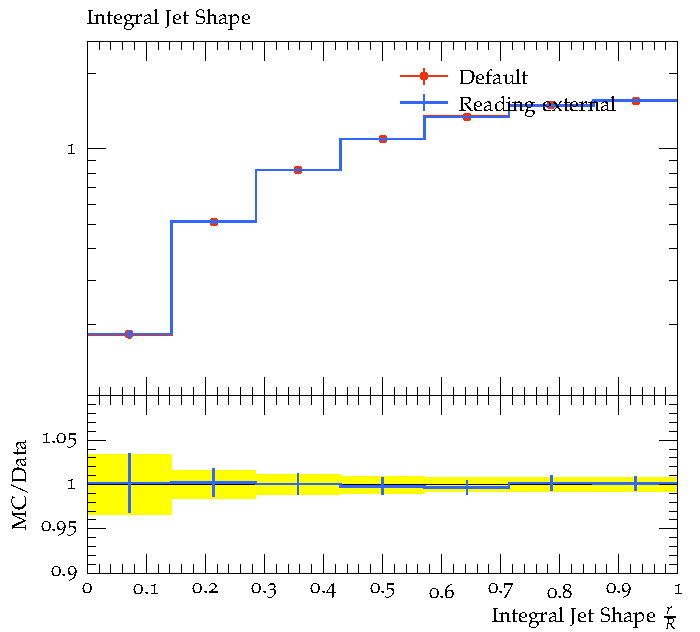
\includegraphics[scale=0.6]{images/Int_shape_read.pdf}        
        \end{minipage}
\end{frame}
\begin{frame}\frametitle{Preliminary Results}

        
        \begin{minipage}{1.0\textwidth}
		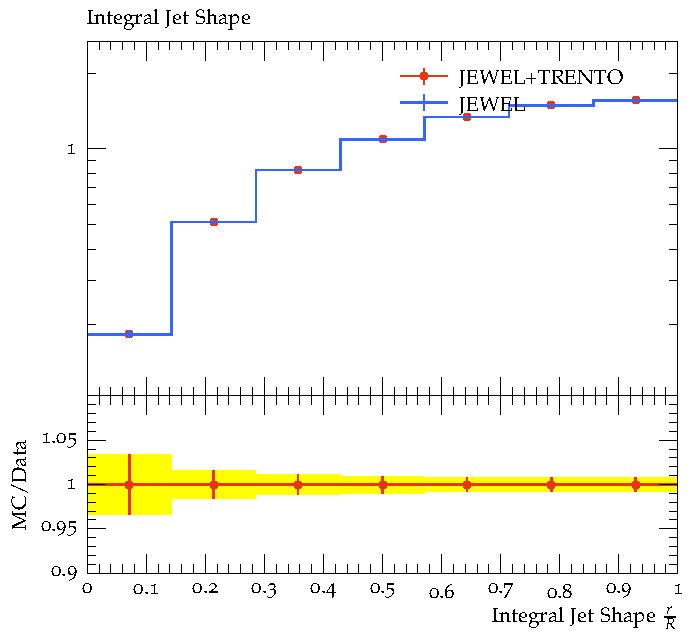
\includegraphics[scale=0.6]{images/Int_shape_trento.pdf}        
        \end{minipage}
\end{frame}


\subsection{Jet mass}

\begin{frame}\frametitle{Preliminary Results}

        
        \begin{minipage}{1.0\textwidth}
		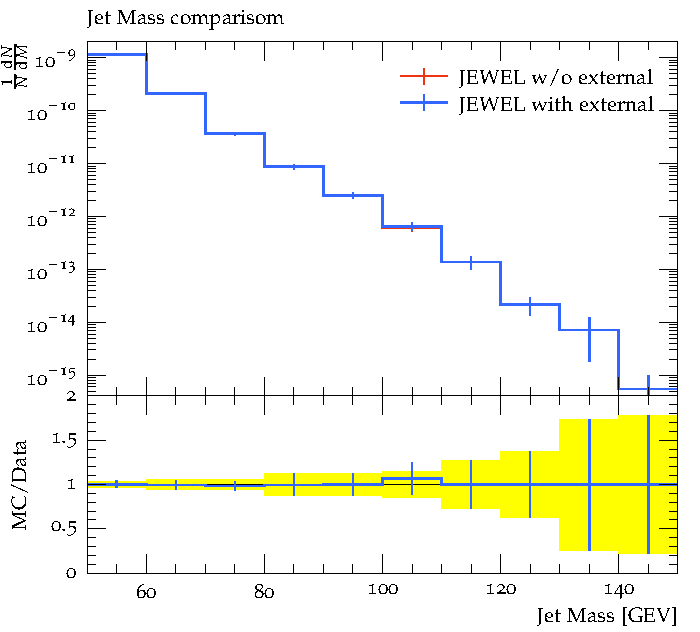
\includegraphics[scale=0.6]{images/Mass_read.pdf}        
        \end{minipage}
\end{frame}

\begin{frame}\frametitle{Preliminary Results}

        
        \begin{minipage}{1.0\textwidth}
		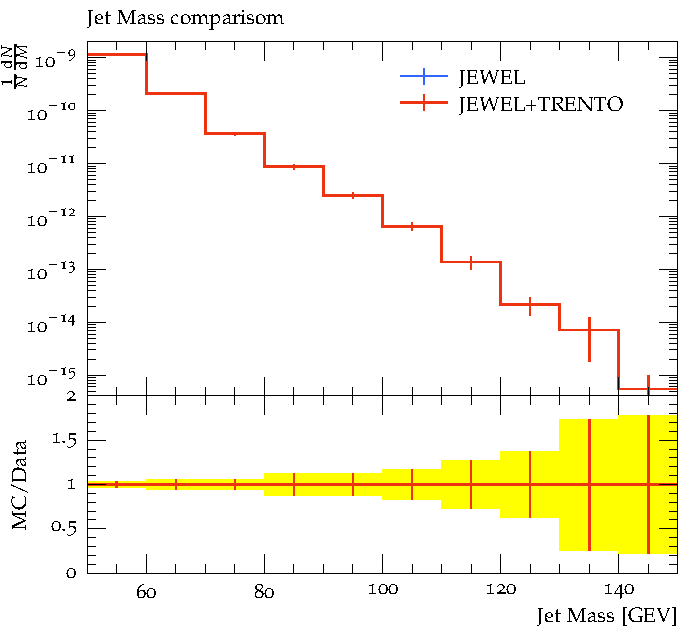
\includegraphics[scale=0.6]{images/Mass_4Mom_trento.pdf}        
        \end{minipage}
\end{frame}

\subsection{Pseudorapidity Distribution of $+/-$ ratio}

\begin{frame}\frametitle{Preliminary Results}

        
        \begin{minipage}{1.0\textwidth}
		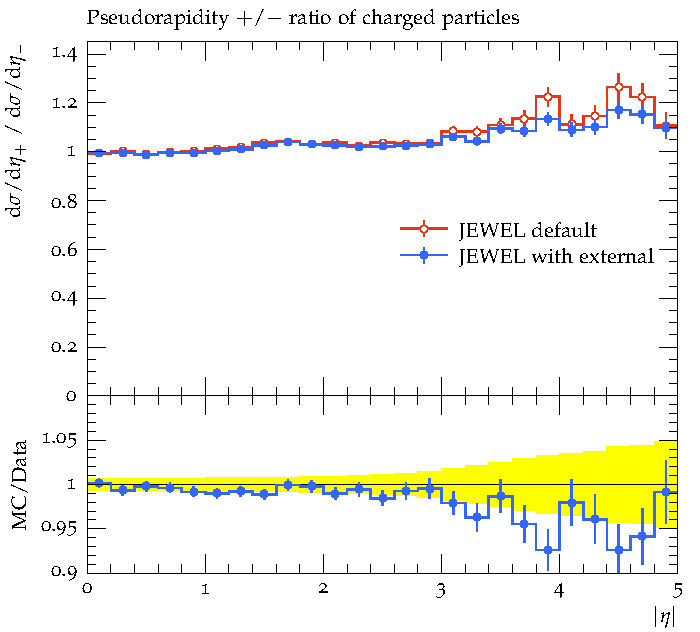
\includegraphics[scale=0.6]{images/Read_EtaChPMRatio.pdf}        
        \end{minipage}
\end{frame}

\begin{frame}\frametitle{Preliminary Results}

        
        \begin{minipage}{1.0\textwidth}
		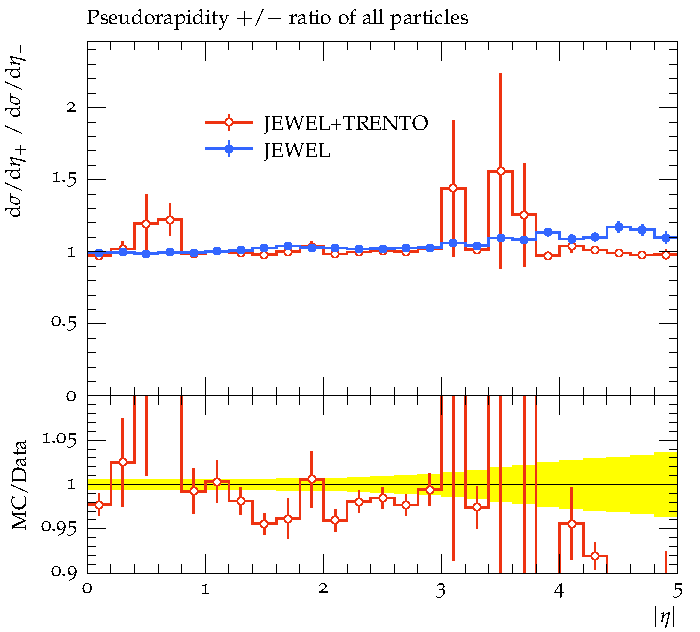
\includegraphics[scale=0.6]{images/trento_EtaPMRatio.pdf}        
        \end{minipage}
\end{frame}

%\begin{frame}\frametitle{What is JEWEL?}
%        JEWEL is a Monte Carlo High Energy generator whose name stands for
%        Jet Evolution with Energy Loss. It propagates partons inside a
%        thermal medium that simulates heavy-ion collisions in accelerators
%        such as RHIC or LHC.
%        \\
%        \pause
%        It accomplishes this by use of a perturbative approach, combining regular parton shower
%        with successive scatterings:
%        \begin{minipage}{1.0\textwidth}
%		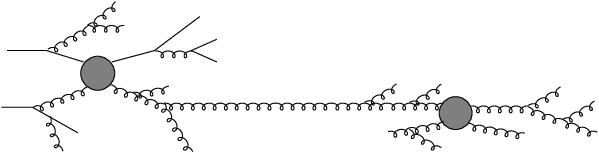
\includegraphics[scale=0.5]{images/feynman.png}        
%        \end{minipage}
%\end{frame}
%
%\subsection{Event Generation}
%\begin{frame}\frametitle{Event Generations}
%	The process of event generation if described by the following:
%	\begin{itemize}
%	\pause
%	\item First, PYTHIA is called to calculate the initial scatterings of the partons inside the
%	nuclei;
%	\pause
%	\item The scattered partons are then propagated through the medium with JEWEL, where the medium
%	is seen by the parton as a collection of scattering centres;
%	\pause
%	\item Once all of the partons have reached the minimum of virtuality, given by an infrared
%	regulator, they are given back to PYTHIA for hadronization;
%	\end{itemize}
%\end{frame}
%
%\subsection{Physics of JEWEL}
%
%\begin{frame}\frametitle{Physics of JEWEL}
%	The use of perturbative approach is dealt with by making use of a probabilistic interpretation
%	of the Sudakov form factor:
%	\begin{equation}
%	S_a(t_h,t_c) = \exp \left\{ -\int_{t_c}^{t_h} \frac{dt}{t} \int_{z_{min}}^{z_{max}} dz \sum_b \frac{\alpha(k_{\bot}^2)}{2\pi} \hat{P}_{ab}(z) \right\}
%	\end{equation}
%	\pause
%	Wich means we can take it as the probability that a parton $a$ emites no resolvable radiation
%	between the scales $t_c$ and $t_h$.
%\end{frame}
%
%\begin{frame}\frametitle{Physics of JEWEL}
%	The Sudakov form factor is used to perform the evolution by enforcing radiation until the
%	parton reaches the $t_c$ \textit{cut-off}.
%	\\ \pause
%	Besides that, the medium, seen as a collection of scattering centers by the parton, also has
%	the probability of interaction.
%	\\ \pause
%	This probability is given by the regular cross-section of a $2 \rightarrow 2$ process,given by:
%	\begin{equation}
%	\sigma_i(E,T)=\int_{0}^{|\hat{t}|_{max}(E,T)}d|\hat{t}|\int_{x_{min}(|\hat{t}|)}^{x_{max}(|\hat{t}|)} dx \sum_{j \in \{ q,\overline{q},g\}} f_{j}^{i}(x,\hat{t})\frac{\mathrm{d}\sigma}{\mathrm{d}\hat{t}}(x\hat{s},|\hat{t}|)
%	\end{equation}
%\end{frame}
%
%\section{Medium Model}
%\subsection{Initial Conditions}
%
%\begin{frame}\frametitle{Initial Conditions}
%	The model employed by JEWEL is a variant of Bjorken model that
%	approachs the initial contitions by the definition of the nuclear thickness 
%	function:
%	\begin{equation}
%	T(x,y) = \int dz \rho(x,y,z)
%	\end{equation}
%\end{frame}
%
%\begin{frame}\frametitle{Initial Conditions}
%	The nuclear thickness functions are then used to define a reduced thickness by:
%	\begin{equation}
%	\begin{split}
%	n(b,x,y) &= T_A(x-\frac{b}{2},y) \left( 1-\exp\left( \sigma_{NN} T_B(x+\frac{b}{2},y) \right) \right) \\
%	&+ T_B(x+\frac{b}{2},y) \left( 1-\exp\left( \sigma_{NN} T_A(x-\frac{b}{2},y) \right) \right)
%	\end{split}
%	\end{equation}
%	Where $\sigma_{NN}$ is the nuclear cross-section and $b$ is the impact parameter.
%\end{frame}
%
%\begin{frame}\frametitle{Initial Conditions}
%	This reduced thickness is then applied to take a map of the initial energy density:
%	\begin{equation}
%	\epsilon(x,y,b,\tau_i) = \epsilon_i \frac{n_{part}(x,y,b)}{<n_{part}>(b=0)}
%	\end{equation}
%	Where $<n_{part}>(b=0) \approx \frac{2 A}{\pi R_A}$.
%\end{frame}
%
%\begin{frame}\frametitle{Initial Conditions}
%	The value of $\epsilon_i$ is determined by an initial temperature given as a parameter to
%	JEWEL. This translation is made through the use of the relation $\epsilon_i \propto T_i^4$.
%\end{frame}
%
%\subsection{Medium Evolution}
%
%\begin{frame}\frametitle{Medium Evolution}
%	The medium evolution is performed analytically by use of:
%	\begin{equation}
%	\epsilon(x,y,b,\tau) = \epsilon_i (x,y,b,\tau_i) \left( \frac{\tau}{\tau_i} \right)^{-\frac{4}{3}}
%	\end{equation}
%	\pause
%	This that the temperature evolves according to:
%	\begin{equation}
%	T(x,y,b,\tau) \propto \epsilon(x,y,b,\tau_i)^{1/4} \left( \frac{\tau}{\tau_i} \right)^{-\frac{4}{3}}
%	\end{equation}
%\end{frame}
%
%\section{Jet Observables}
%\subsection{JetAlgorithms}
%
%\begin{frame}\frametitle{Jet Algorithms}
%	Today, the main type of algorithm to cluster particles from a given event into jets,
%	thus defining a jet, are the sequential recombination algorithms. They define a distance
%	functions between particles:
%	\pause
%	\begin{equation}
%	d_{ij} = \min(p_{ti}^{2p},p_{tj}^{2p}) \frac{\Delta R_{ij}^2}{R^2}
%	\end{equation}
%	\pause
%	Then a process of iteration is realized, where the particles with minimum $d_{ij}$ are
%	combined to form the given jets.
%\end{frame}
%
%\begin{frame}\frametitle{Jet Algorithms}
%	Once the jets are found, one class of the possible observables are the jet shape observables.
%	\pause
%	\\
%	These reflect mush of the evolution that occurs in the jet formation, as well as
%	the process of hadronization.
%\end{frame}
%
%\subsection{SoftDrop Procedure}
%
%\begin{frame}\frametitle{SoftDrop Procedure}
%	One form of extracting information about jet shape is through the SoftDrop Procedure.
%	\pause
%	\\
%	This is done by undoing the last step of the jet recombination.
%	\pause
%	\\
%	The SoftDrop condition is:
%	\begin{equation}
%	\frac{\min(p_{T1},p_{T2})}{p_{T1}+p_{T2}} > z_{cut} \left(\frac{\Delta R_{12}}{R_0}\right)^{\beta}
%	\end{equation}
%\end{frame}
%
%\begin{frame}\frametitle{SoftDrop Procedure}
%	Once the condition has been applied, the quantity:
%	\begin{equation}
%	\frac{\min(p_{T1},p_{T2})}{p_{T1}+p_{T2}}
%	\end{equation}
%	Reflects an observable that is usually related to the first splitting of the parent parton.
%	\pause
%	\\
%	This can be seen in the results of the fact that they follow the Altarelli-Parisi splitting
%	functions.
%\end{frame}
%
%\section{JEWEL Results}
%\subsection{JEWEL Validation}
%
%\begin{frame}\frametitle{JEWEL Validation}
%    \begin{minipage}{1\textwidth}
%	The validation of JEWEL has been performed by comparing with exepriments such as:    
%    \end{minipage}
%    \begin{columns}
%    \begin{column}{0.5\textwidth}
%	\begin{minipage}[l]{0.5\textwidth}
%	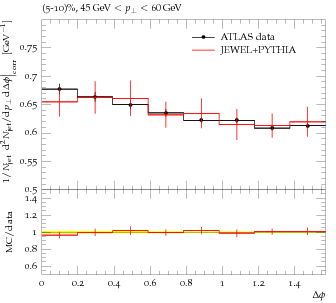
\includegraphics[scale=0.5]{images/atlas_jewel.png}
%	\end{minipage}
%	\end{column}
%    \begin{column}{0.5\textwidth}
%	\begin{minipage}[r]{1\textwidth}
%	Centrality dependence of the angular distribution of single inclusive jets in Pb+Pb collisions
%	at $\sqrt{s_{NN}}=2.76\mathrm{TeV}$ for a jet radius $R=0.2$ and $|\eta_{jet}|<2.1$ in the
%	range $45\mathrm{GeV}<p_t<60\mathrm{GeV}$.
%	\end{minipage}
%	\end{column}
%	\end{columns}
%\end{frame}
%
%\begin{frame}\frametitle{JEWEL Validation}
%    \begin{minipage}{1\textwidth}
%	The validation of JEWEL has been performed by comparing with exepriments such as:    
%    \end{minipage}
%    \begin{columns}
%    \begin{column}{0.5\textwidth}
%	\begin{minipage}[l]{0.5\textwidth}
%	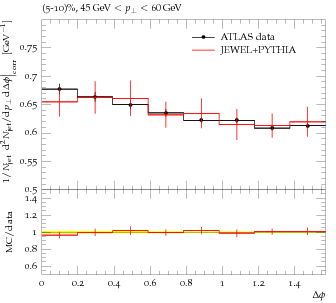
\includegraphics[scale=0.5]{images/atlas_jewel.png}
%	\end{minipage}
%	\end{column}
%    \begin{column}{0.5\textwidth}
%	\begin{minipage}[r]{1\textwidth}
%	Centrality dependence of the angular distribution of single inclusive jets in Pb+Pb collisions
%	at $\sqrt{s_{NN}}=2.76\mathrm{TeV}$ for a jet radius $R=0.2$ and $|\eta_{jet}|<2.1$ in the
%	range $45\mathrm{GeV}<p_t<60\mathrm{GeV}$.
%	\end{minipage}
%	\end{column}
%	\end{columns}
%\end{frame}
%
%\begin{frame}\frametitle{JEWEL Validation}
%    \begin{minipage}{1\textwidth}
%	The validation of JEWEL has been performed by comparing with exepriments such as:    
%    \end{minipage}
%    \begin{columns}
%    \begin{column}{0.5\textwidth}
%	\begin{minipage}[l]{0.5\textwidth}
%	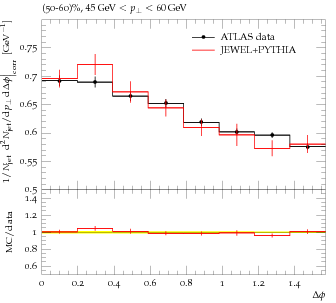
\includegraphics[scale=0.5]{images/atlas_jewel_1.png}
%	\end{minipage}
%	\end{column}
%    \begin{column}{0.5\textwidth}
%	\begin{minipage}[r]{1\textwidth}
%	Centrality dependence of the angular distribution of single inclusive jets in Pb+Pb collisions
%	at $\sqrt{s_{NN}}=2.76\mathrm{TeV}$ for a jet radius $R=0.2$ and $|\eta_{jet}|<2.1$ in the
%	range $45\mathrm{GeV}<p_t<60\mathrm{GeV}$.
%	\end{minipage}
%	\end{column}
%	\end{columns}
%\end{frame}
%
%\begin{frame}\frametitle{JEWEL Validation}
%    \begin{minipage}{1\textwidth}
%	The validation of JEWEL has been performed by comparing with exepriments such as:    
%    \end{minipage}
%    \begin{columns}
%    \begin{column}{0.5\textwidth}
%	\begin{minipage}[l]{0.5\textwidth}
%	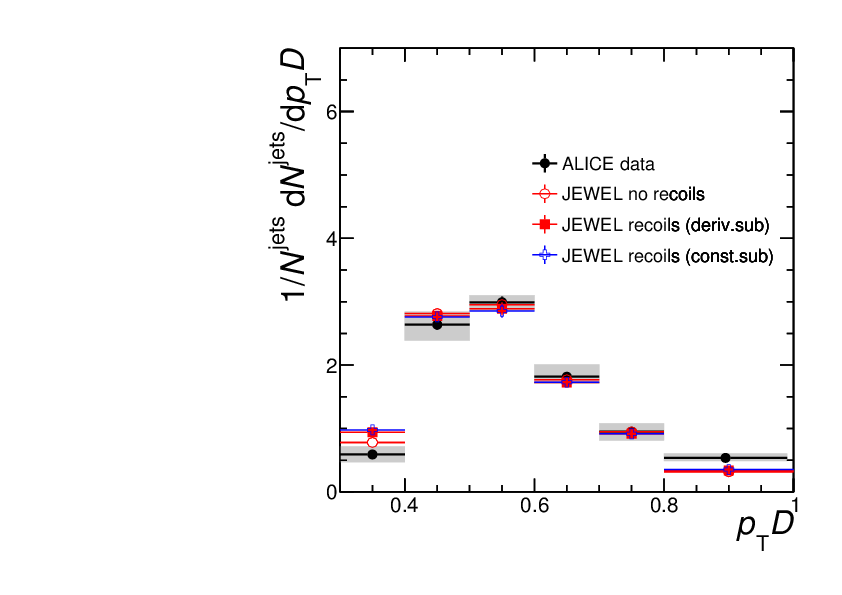
\includegraphics[scale=0.2]{images/alice_jewel.png}
%	\end{minipage}
%	\end{column}
%    \begin{column}{0.5\textwidth}
%	\begin{minipage}[r]{1\textwidth}
%	Jet shape distributions in $0\backsim10$ central PbPb collisions at $\sqrt{s_{NN}}=2.76\mathrm{TeV}$ for $R=0.2$ in range of jet $p_{chT}$,jet of $40\backsim60\mathrm{GeV}/c$ compared to JEWEL with and without recoils with different subtraction methods. The coloured boxes represent the experimental uncertainty on the jet shapes.
%	\end{minipage}
%	\end{column}
%	\end{columns}
%\end{frame}
%
%\section{What to do with JEWEL?}
%\subsection{What to do with JEWEL?}
%
%\begin{frame}\frametitle{What to do with JEWEL?}
%	The steps suggested of what to do next with JEWEL are:
%	\begin{itemize}
%	\pause
%	\item Prepare a code to read external medium files(currently running);
%	\pause
%	\item Couple it with a different model of initial conditions(currently running with TRENTO);
%	\pause
%	\item Couple it with a more realistic hydro;
%	\pause
%	\item Talk to JEWEL developers to adapt it to run with haevy partons;
%	\end{itemize}
%\end{frame}
%
%\begin{frame}\frametitle{What is JEWEL?}
%        JEWEL is a Monte Carlo High Energy generator whose name stands for
%        Jet Evolution with Energy Loss. It propagates partons inside a
%        thermal medium that simulates heavy-ion collisions in accelerators
%        such as RHIC or LHC.
%        \\
%        \pause
%        It accomplishes this by use of a perturbative approach, combining regular parton shower
%        with successive scatterings:
%        \begin{minipage}{1.0\textwidth}
%		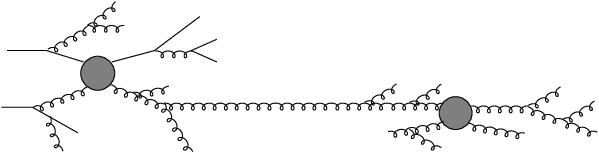
\includegraphics[scale=0.5]{images/feynman.png}        
%        \end{minipage}
%\end{frame}
%
%\subsection{Event Generation}
%\begin{frame}\frametitle{Event Generations}
%	The process of event generation if described by the following:
%	\begin{itemize}
%	\pause
%	\item First, PYTHIA is called to calculate the initial scatterings of the partons inside the
%	nuclei;
%	\pause
%	\item The scattered partons are then propagated through the medium with JEWEL, where the medium
%	is seen by the parton as a collection of scattering centres;
%	\pause
%	\item Once all of the partons have reached the minimum of virtuality, given by an infrared
%	regulator, they are given back to PYTHIA for hadronization;
%	\end{itemize}
%\end{frame}
%
%\subsection{Physics of JEWEL}
%
%\begin{frame}\frametitle{Physics of JEWEL}
%	The use of perturbative approach is dealt with by making use of a probabilistic interpretation
%	of the Sudakov form factor:
%	\begin{equation}
%	S_a(t_h,t_c) = \exp \left\{ -\int_{t_c}^{t_h} \frac{dt}{t} \int_{z_{min}}^{z_{max}} dz \sum_b \frac{\alpha(k_{\bot}^2)}{2\pi} \hat{P}_{ab}(z) \right\}
%	\end{equation}
%	\pause
%	Wich means we can take it as the probability that a parton $a$ emites no resolvable radiation
%	between the scales $t_c$ and $t_h$.
%\end{frame}
%
%\begin{frame}\frametitle{Physics of JEWEL}
%	The Sudakov form factor is used to perform the evolution by enforcing radiation until the
%	parton reaches the $t_c$ \textit{cut-off}.
%	\\ \pause
%	Besides that, the medium, seen as a collection of scattering centers by the parton, also has
%	the probability of interaction.
%	\\ \pause
%	This probability is given by the regular cross-section of a $2 \rightarrow 2$ process,given by:
%	\begin{equation}
%	\sigma_i(E,T)=\int_{0}^{|\hat{t}|_{max}(E,T)}d|\hat{t}|\int_{x_{min}(|\hat{t}|)}^{x_{max}(|\hat{t}|)} dx \sum_{j \in \{ q,\overline{q},g\}} f_{j}^{i}(x,\hat{t})\frac{\mathrm{d}\sigma}{\mathrm{d}\hat{t}}(x\hat{s},|\hat{t}|)
%	\end{equation}
%\end{frame}
%
%\section{Medium Model}
%\subsection{Initial Conditions}
%
%\begin{frame}\frametitle{Initial Conditions}
%	The model employed by JEWEL is a variant of Bjorken model that
%	approachs the initial contitions by the definition of the nuclear thickness 
%	function:
%	\begin{equation}
%	T(x,y) = \int dz \rho(x,y,z)
%	\end{equation}
%\end{frame}
%
%\begin{frame}\frametitle{Initial Conditions}
%	The nuclear thickness functions are then used to define a reduced thickness by:
%	\begin{equation}
%	\begin{split}
%	n(b,x,y) &= T_A(x-\frac{b}{2},y) \left( 1-\exp\left( \sigma_{NN} T_B(x+\frac{b}{2},y) \right) \right) \\
%	&+ T_B(x+\frac{b}{2},y) \left( 1-\exp\left( \sigma_{NN} T_A(x-\frac{b}{2},y) \right) \right)
%	\end{split}
%	\end{equation}
%	Where $\sigma_{NN}$ is the nuclear cross-section and $b$ is the impact parameter.
%\end{frame}
%
%\begin{frame}\frametitle{Initial Conditions}
%	This reduced thickness is then applied to take a map of the initial energy density:
%	\begin{equation}
%	\epsilon(x,y,b,\tau_i) = \epsilon_i \frac{n_{part}(x,y,b)}{<n_{part}>(b=0)}
%	\end{equation}
%	Where $<n_{part}>(b=0) \approx \frac{2 A}{\pi R_A}$.
%\end{frame}
%
%\begin{frame}\frametitle{Initial Conditions}
%	The value of $\epsilon_i$ is determined by an initial temperature given as a parameter to
%	JEWEL. This translation is made through the use of the relation $\epsilon_i \propto T_i^4$.
%\end{frame}
%
%\subsection{Medium Evolution}
%
%\begin{frame}\frametitle{Medium Evolution}
%	The medium evolution is performed analytically by use of:
%	\begin{equation}
%	\epsilon(x,y,b,\tau) = \epsilon_i (x,y,b,\tau_i) \left( \frac{\tau}{\tau_i} \right)^{-\frac{4}{3}}
%	\end{equation}
%	\pause
%	This that the temperature evolves according to:
%	\begin{equation}
%	T(x,y,b,\tau) \propto \epsilon(x,y,b,\tau_i)^{1/4} \left( \frac{\tau}{\tau_i} \right)^{-\frac{4}{3}}
%	\end{equation}
%\end{frame}
%
%\section{Jet Observables}
%\subsection{JetAlgorithms}
%
%\begin{frame}\frametitle{Jet Algorithms}
%	Today, the main type of algorithm to cluster particles from a given event into jets,
%	thus defining a jet, are the sequential recombination algorithms. They define a distance
%	functions between particles:
%	\pause
%	\begin{equation}
%	d_{ij} = \min(p_{ti}^{2p},p_{tj}^{2p}) \frac{\Delta R_{ij}^2}{R^2}
%	\end{equation}
%	\pause
%	Then a process of iteration is realized, where the particles with minimum $d_{ij}$ are
%	combined to form the given jets.
%\end{frame}
%
%\begin{frame}\frametitle{Jet Algorithms}
%	Once the jets are found, one class of the possible observables are the jet shape observables.
%	\pause
%	\\
%	These reflect mush of the evolution that occurs in the jet formation, as well as
%	the process of hadronization.
%\end{frame}
%
%\subsection{SoftDrop Procedure}
%
%\begin{frame}\frametitle{SoftDrop Procedure}
%	One form of extracting information about jet shape is through the SoftDrop Procedure.
%	\pause
%	\\
%	This is done by undoing the last step of the jet recombination.
%	\pause
%	\\
%	The SoftDrop condition is:
%	\begin{equation}
%	\frac{\min(p_{T1},p_{T2})}{p_{T1}+p_{T2}} > z_{cut} \left(\frac{\Delta R_{12}}{R_0}\right)^{\beta}
%	\end{equation}
%\end{frame}
%
%\begin{frame}\frametitle{SoftDrop Procedure}
%	Once the condition has been applied, the quantity:
%	\begin{equation}
%	\frac{\min(p_{T1},p_{T2})}{p_{T1}+p_{T2}}
%	\end{equation}
%	Reflects an observable that is usually related to the first splitting of the parent parton.
%	\pause
%	\\
%	This can be seen in the results of the fact that they follow the Altarelli-Parisi splitting
%	functions.
%\end{frame}
%
%\section{JEWEL Results}
%\subsection{JEWEL Validation}
%
%\begin{frame}\frametitle{JEWEL Validation}
%    \begin{minipage}{1\textwidth}
%	The validation of JEWEL has been performed by comparing with exepriments such as:    
%    \end{minipage}
%    \begin{columns}
%    \begin{column}{0.5\textwidth}
%	\begin{minipage}[l]{0.5\textwidth}
%	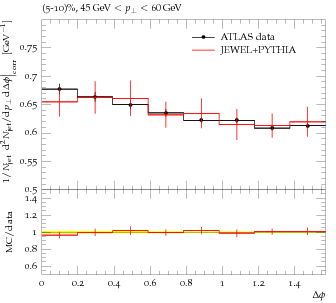
\includegraphics[scale=0.5]{images/atlas_jewel.png}
%	\end{minipage}
%	\end{column}
%    \begin{column}{0.5\textwidth}
%	\begin{minipage}[r]{1\textwidth}
%	Centrality dependence of the angular distribution of single inclusive jets in Pb+Pb collisions
%	at $\sqrt{s_{NN}}=2.76\mathrm{TeV}$ for a jet radius $R=0.2$ and $|\eta_{jet}|<2.1$ in the
%	range $45\mathrm{GeV}<p_t<60\mathrm{GeV}$.
%	\end{minipage}
%	\end{column}
%	\end{columns}
%\end{frame}
%
%\begin{frame}\frametitle{JEWEL Validation}
%    \begin{minipage}{1\textwidth}
%	The validation of JEWEL has been performed by comparing with exepriments such as:    
%    \end{minipage}
%    \begin{columns}
%    \begin{column}{0.5\textwidth}
%	\begin{minipage}[l]{0.5\textwidth}
%	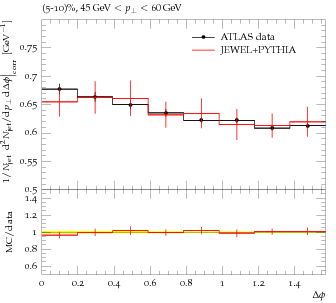
\includegraphics[scale=0.5]{images/atlas_jewel.png}
%	\end{minipage}
%	\end{column}
%    \begin{column}{0.5\textwidth}
%	\begin{minipage}[r]{1\textwidth}
%	Centrality dependence of the angular distribution of single inclusive jets in Pb+Pb collisions
%	at $\sqrt{s_{NN}}=2.76\mathrm{TeV}$ for a jet radius $R=0.2$ and $|\eta_{jet}|<2.1$ in the
%	range $45\mathrm{GeV}<p_t<60\mathrm{GeV}$.
%	\end{minipage}
%	\end{column}
%	\end{columns}
%\end{frame}
%
%\begin{frame}\frametitle{JEWEL Validation}
%    \begin{minipage}{1\textwidth}
%	The validation of JEWEL has been performed by comparing with exepriments such as:    
%    \end{minipage}
%    \begin{columns}
%    \begin{column}{0.5\textwidth}
%	\begin{minipage}[l]{0.5\textwidth}
%	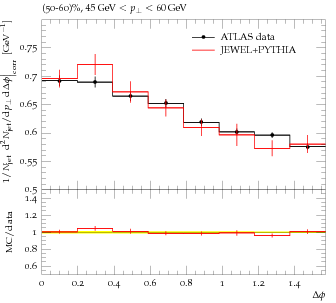
\includegraphics[scale=0.5]{images/atlas_jewel_1.png}
%	\end{minipage}
%	\end{column}
%    \begin{column}{0.5\textwidth}
%	\begin{minipage}[r]{1\textwidth}
%	Centrality dependence of the angular distribution of single inclusive jets in Pb+Pb collisions
%	at $\sqrt{s_{NN}}=2.76\mathrm{TeV}$ for a jet radius $R=0.2$ and $|\eta_{jet}|<2.1$ in the
%	range $45\mathrm{GeV}<p_t<60\mathrm{GeV}$.
%	\end{minipage}
%	\end{column}
%	\end{columns}
%\end{frame}
%
%\begin{frame}\frametitle{JEWEL Validation}
%    \begin{minipage}{1\textwidth}
%	The validation of JEWEL has been performed by comparing with exepriments such as:    
%    \end{minipage}
%    \begin{columns}
%    \begin{column}{0.5\textwidth}
%	\begin{minipage}[l]{0.5\textwidth}
%	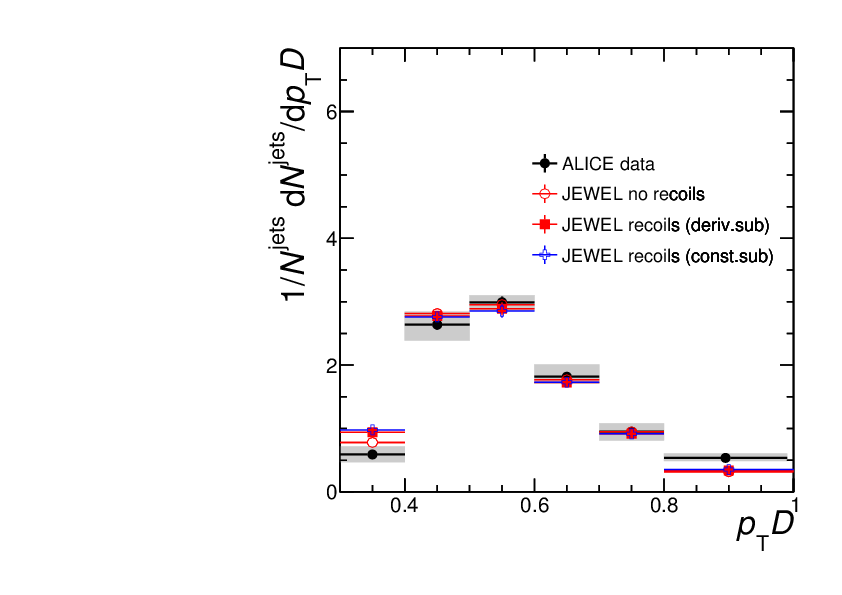
\includegraphics[scale=0.2]{images/alice_jewel.png}
%	\end{minipage}
%	\end{column}
%    \begin{column}{0.5\textwidth}
%	\begin{minipage}[r]{1\textwidth}
%	Jet shape distributions in $0\backsim10$ central PbPb collisions at $\sqrt{s_{NN}}=2.76\mathrm{TeV}$ for $R=0.2$ in range of jet $p_{chT}$,jet of $40\backsim60\mathrm{GeV}/c$ compared to JEWEL with and without recoils with different subtraction methods. The coloured boxes represent the experimental uncertainty on the jet shapes.
%	\end{minipage}
%	\end{column}
%	\end{columns}
%\end{frame}
%
%\section{What to do with JEWEL?}
%\subsection{What to do with JEWEL?}
%
%\begin{frame}\frametitle{What to do with JEWEL?}
%	The steps suggested of what to do next with JEWEL are:
%	\begin{itemize}
%	\pause
%	\item Prepare a code to read external medium files(currently running);
%	\pause
%	\item Couple it with a different model of initial conditions(currently running with TRENTO);
%	\pause
%	\item Couple it with a more realistic hydro;
%	\pause
%	\item Talk to JEWEL developers to adapt it to run with haevy partons;
%	\end{itemize}
%\end{frame}
%

\end{document}
